\subsection{Avaliação Preliminar do Motor Analítico (Março/2026)}

Um estudo preliminar (março de 2026) avaliou o desempenho bruto do Apache Druid sobre \textasciitilde{}3,1 milhões de registros do INPE. Naquela etapa inicial do projeto, a arquitetura Silver ainda não havia sido desenvolvida. Portanto, o cenário operava exclusivamente com filtros tabulares simples sobre a tabela fato crua, sem o gargalo matemático das intersecções espaciais complexas (GeoJSON).

O experimento submeteu 6 \textit{queries} de referência a diferentes alocações de CPU (2, 4 e 6 núcleos) em dois cenários opostos: estado bruto de ingestão (fragmentado em 6.518 \textit{Tiny Segments}) e estado compactado (granularidade \texttt{YEAR}).

A Figura \ref{fig:abismo_desempenho} sintetiza o impacto estrutural. No estado fragmentado, o sistema atingiu um teto de I/O em \textasciitilde{}1.624ms mesmo com 6 núcleos, evidenciando a Lei de Amdahl perante o \textit{overhead} de 6.518 \textit{file handles}. Em contraste, a simples compactação despencou a latência média para \textasciitilde{}55ms. Mantendo o mesmo hardware, a aceleração chegou a quase 39 vezes no cenário de 4 núcleos. Com o disco organizado, todas as consultas passaram a responder em sub-100ms utilizando apenas 2 núcleos (Figura \ref{fig:barras_compactado}).

\begin{figure}[H]
    \centering
    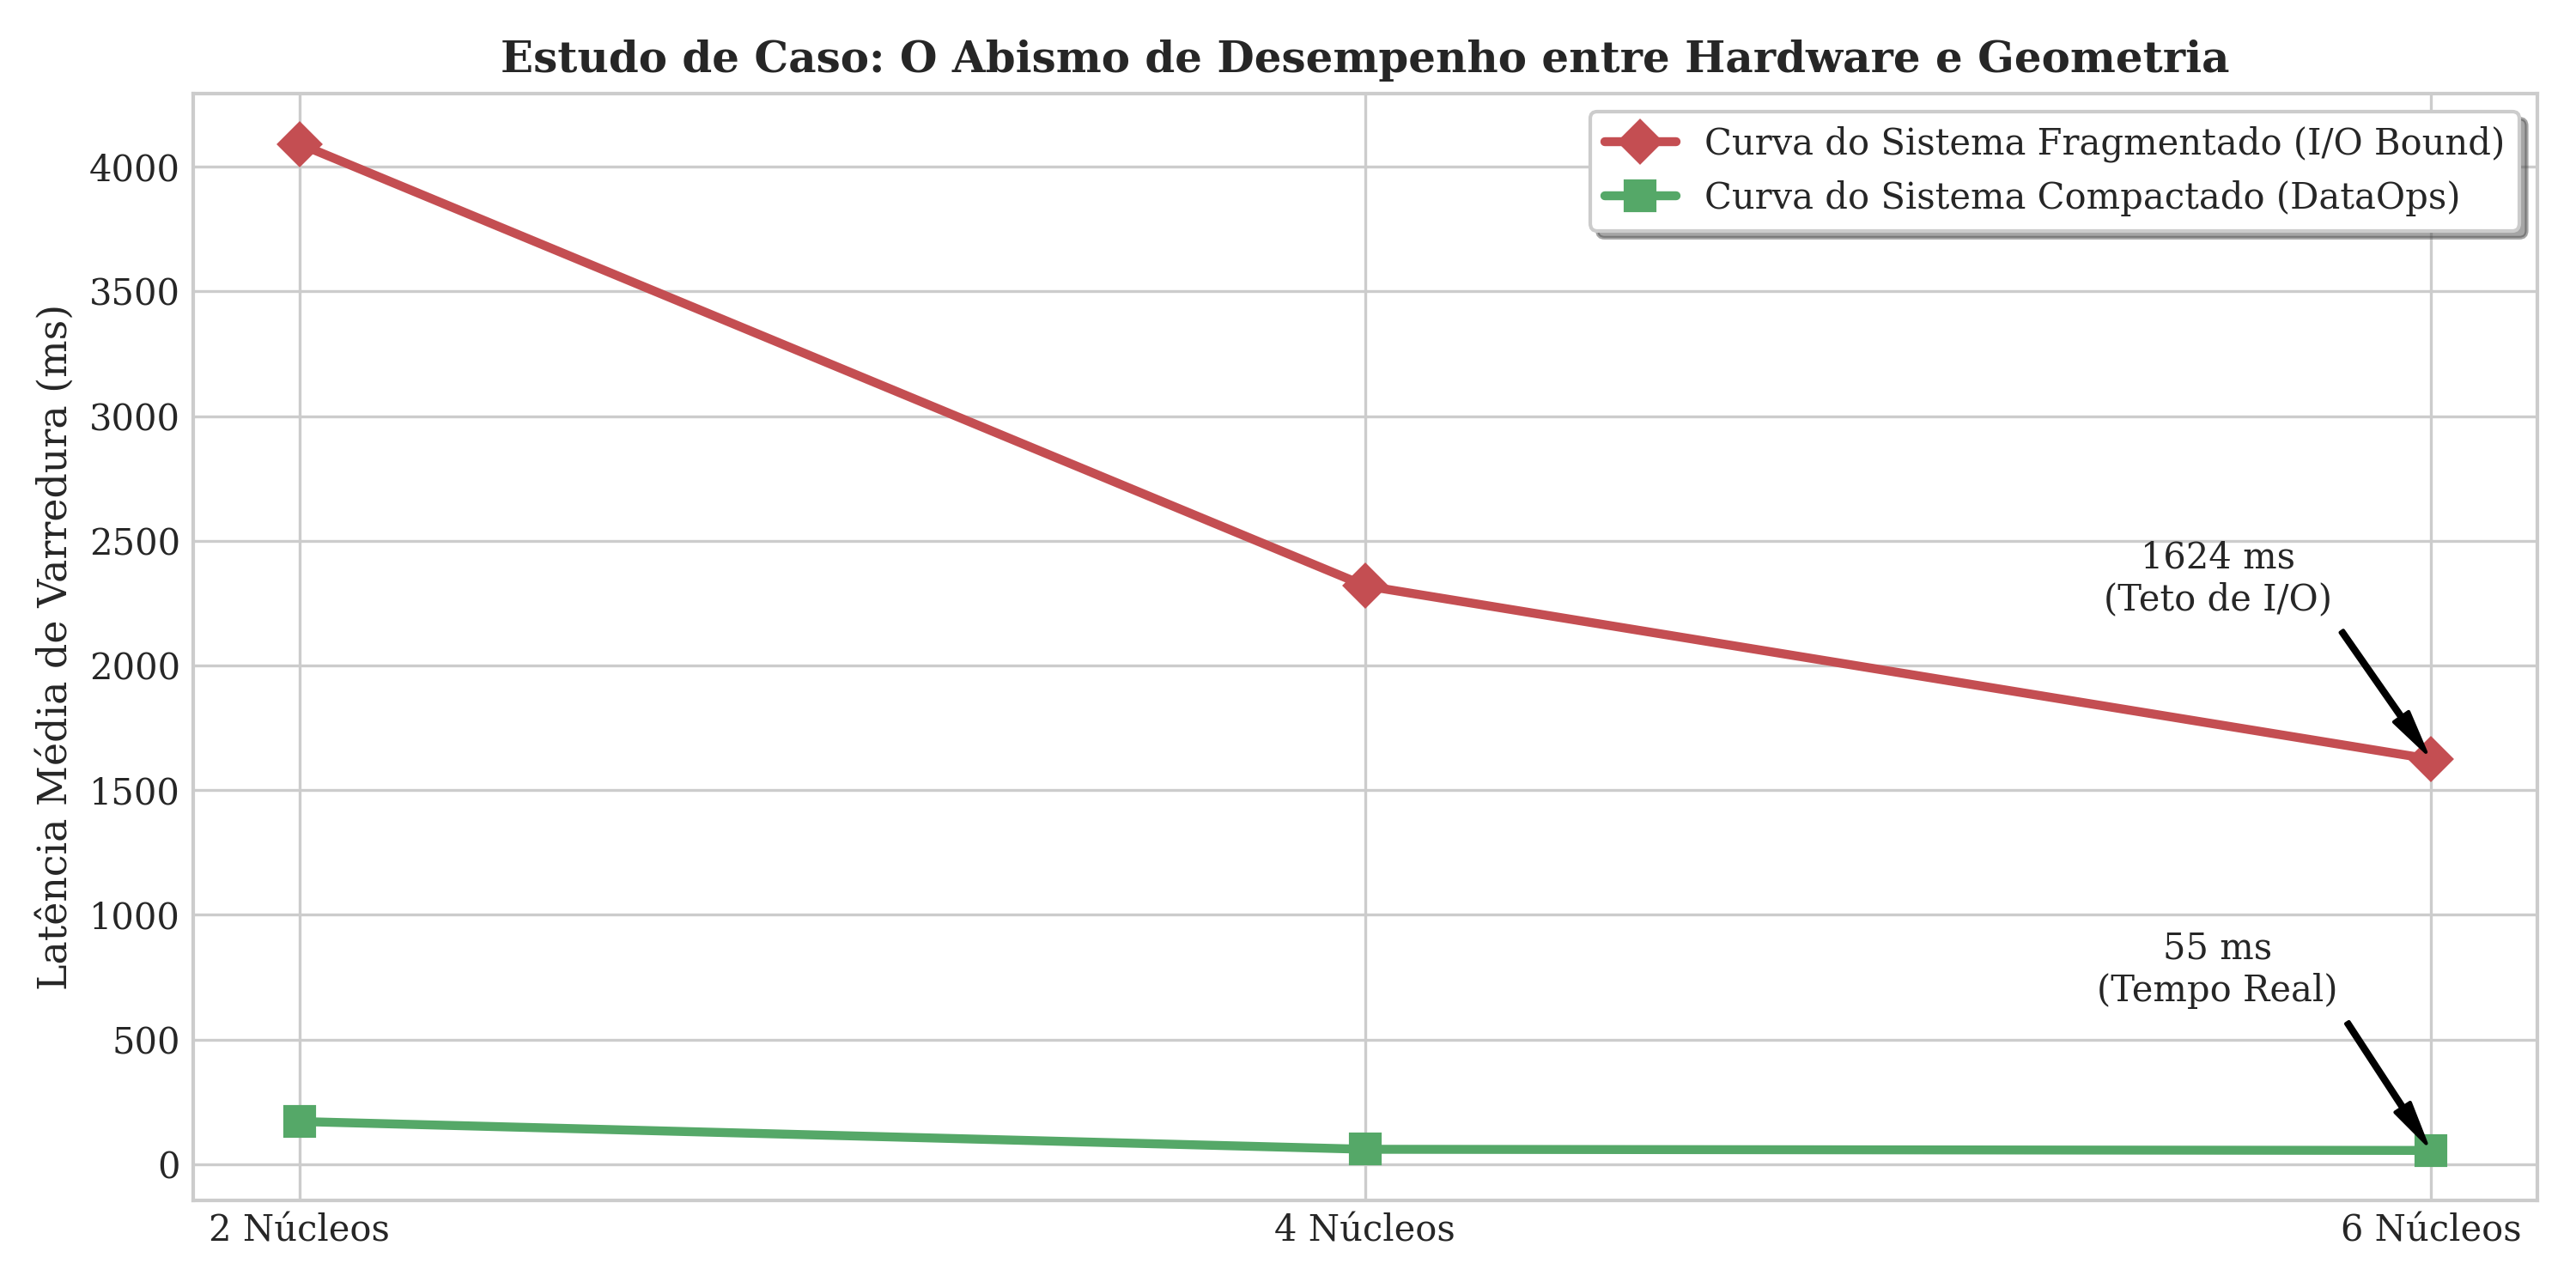
\includegraphics[width=0.85\textwidth]{materiais_apoio/figures/benchmark_preliminar/r3_comparativo_latencia_geral.png}
    \caption{Comparativo de Desempenho: Dados Fragmentados vs. Compactados.}
    \label{fig:abismo_desempenho}
\end{figure}

A Tabela \ref{tab:fator_dataops} quantifica a magnitude dessa otimização. A intervenção algorítmica revelou-se sistematicamente superior à infraestrutura física: o sistema estrangulado a 2 núcleos lendo a base compactada (171ms) foi, na prática, \textbf{\textasciitilde{}9,5 vezes} mais rápido do que o hospedeiro em potência máxima (6 núcleos) tentando processar o caos estrutural (1.624ms).

\begin{table}[H]
    \centering
    \footnotesize
    \caption{Redução de Latência Relativa por Alocação de CPU.}
    \label{tab:fator_dataops}
    \begin{tabular}{lccc}
        \toprule
        \textbf{Hardware} & \textbf{Cold Start (Frag.)} & \textbf{Cold Start (Comp.)} & \textbf{Aceleração} \\
        \midrule
        2 Núcleos & 4.092 ms & 171 ms & 23,9$\times$ \\
        4 Núcleos & 2.320 ms & 60 ms  & 38,8$\times$ \\
        6 Núcleos & 1.624 ms & 55 ms  & 29,4$\times$ \\
        \bottomrule
    \end{tabular}
\end{table}

\begin{figure}[H]
    \centering
    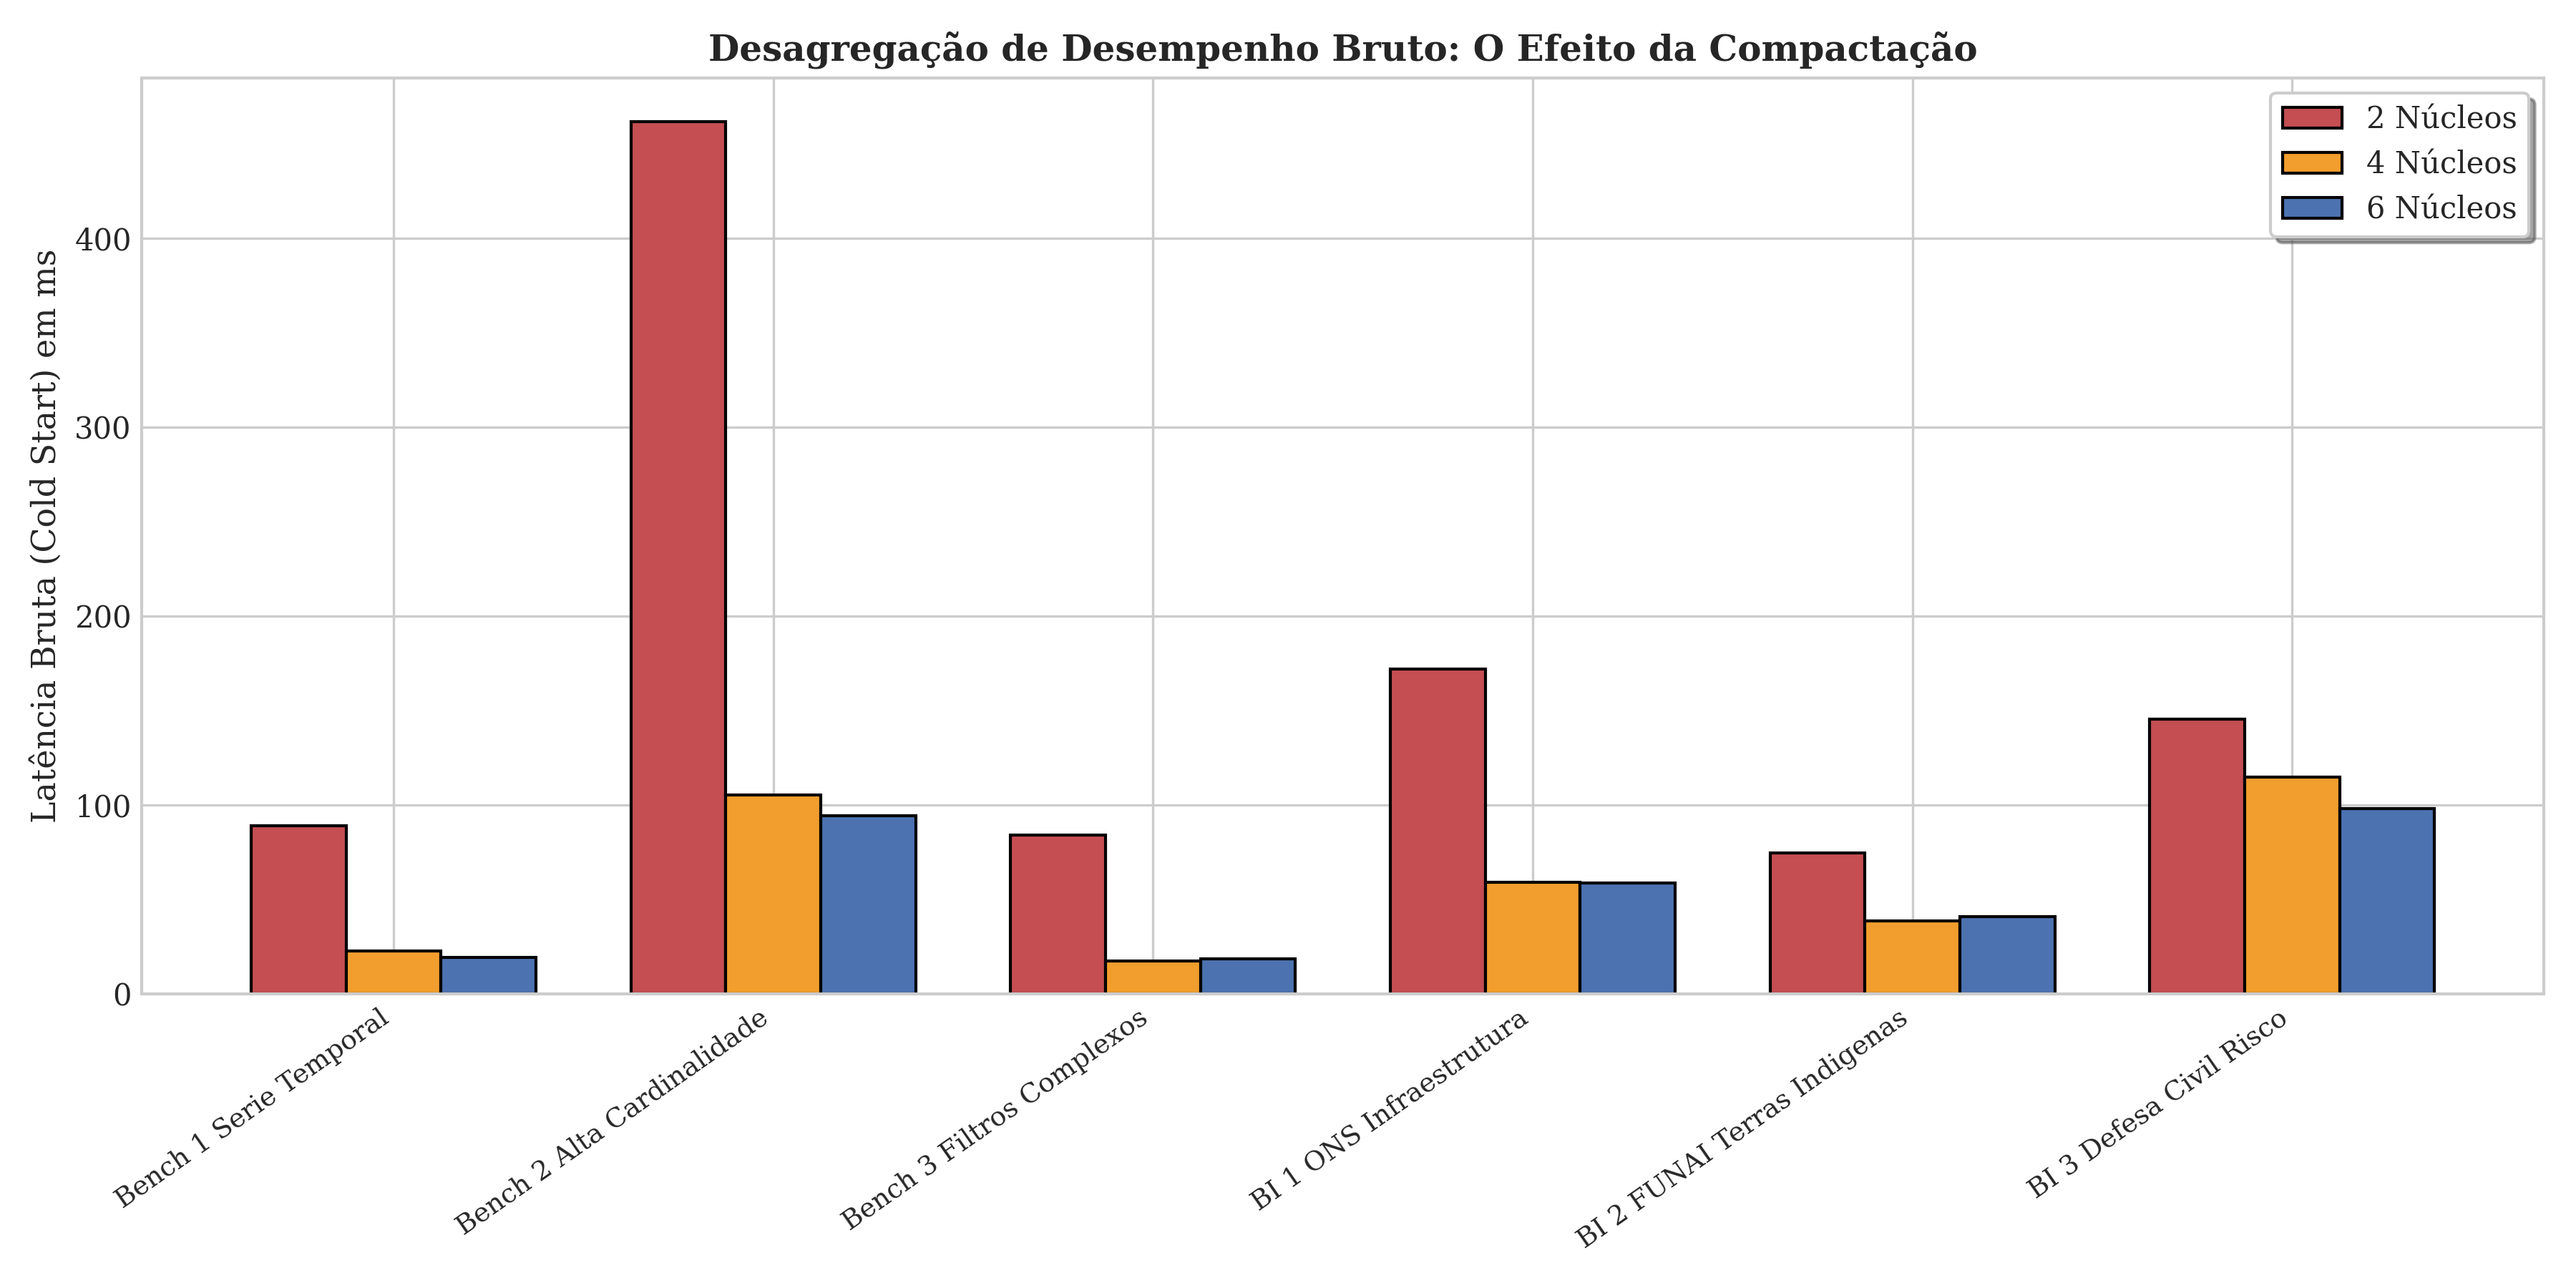
\includegraphics[width=0.85\textwidth]{materiais_apoio/figures/benchmark_preliminar/r2_latencia_por_cpu_compactado.png}
    \caption{Latência por Domínio de Consulta após Compactação (Março/2026).}
    \label{fig:barras_compactado}
\end{figure}
